\documentclass[conference, 10pt]{IEEEtran}
\IEEEoverridecommandlockouts
% The preceding line is only needed to identify funding in the first footnote. If that is unneeded, please comment it out.
\usepackage{cite}
\usepackage{amsmath,amssymb,amsfonts}
\usepackage{algorithmic}
\usepackage{graphicx}
\usepackage{textcomp}
\usepackage{xcolor}
\usepackage{orcidlink}
\usepackage{subcaption}
\usepackage{makecell}
\usepackage[none]{hyphenat}
\usepackage{flushend}
\makeatletter
\newcommand{\linebreakand}{%
\end{@IEEEauthorhalign}
\hfill\mbox{}\par
\mbox{}\hfill\begin{@IEEEauthorhalign}
}
\makeatother
\begin{document}

\title{\textbf{Voice-Based Age and Gender Recognition: A Comparative Study of CNNs, LSTM, BiLSTM, and RezoNet Architecture}\\
}
\author{
\IEEEauthorblockN{1\textsuperscript{st} Minh Nhut Nguyen \orcidlink{0009-0003-1281-5346}}
\IEEEauthorblockA{\textit{Dept. of Artificial Intelligence} \\
\textit{FPT University}\\
Ho Chi Minh City, Vietnam \\
nhutnmse184534@fpt.edu.vn}
\\
\IEEEauthorblockN{3\textsuperscript{rd} Hua Hiep Nguyen \orcidlink{0009-0007-0848-0968}}
\IEEEauthorblockA{\textit{Dept. of Artificial Intelligence} \\
\textit{FPT University}\\
Ho Chi Minh City, Vietnam \\
hiepnhse183787@fpt.edu.vn}
\and
\IEEEauthorblockN{2\textsuperscript{nd} Thanh Trung Nguyen \orcidlink{0009-0004-7553-4848}}
\IEEEauthorblockA{\textit{Dept. of Artificial Intelligence} \\
\textit{FPT University}\\
Ho Chi Minh City, Vietnam \\
trungnt180355@fpt.edu.vn}
\\
\IEEEauthorblockN{4\textsuperscript{th} Dinh Hung Trinh}
\IEEEauthorblockA{\textit{Dept. of Artificial Intelligence} \\
\textit{FPT University}\\
Ho Chi Minh City, Vietnam \\
hungtdse173408@fpt.edu.vn}
}



\maketitle

\begin{abstract}
Abtract
\end{abstract}

\begin{IEEEkeywords}
keyword 1, keyword 2
\end{IEEEkeywords}

\section{Introduction}          %--Chưa add SVM vào nhá
Voice-based recognition systems have become an essential element in various applications, ranging from security systems and customer service automation to personalized user experiences. Among these applications, the ability to accurately determine a speaker's age and gender from voice recordings is particularly valuable for enhancing user interaction and tailoring services more effectively. This research undertakes a comparative analysis of several deep learning architectures—Convolutional Neural Networks (CNNs)~\cite{chua1998cnn}, Long Short-Term Memory networks (LSTMs)~\cite{smagulova2019survey}, Bidirectional LSTMs (BiLSTMs)~\cite{siami2019performance}, and the recently introduced RezoNet architecture—for the task of age and gender recognition from voice data~\cite{hanifa2021review}.

The complexity of voice-based age and gender recognition arises from the need to capture subtle features of vocal signals that vary significantly across different demographics. Traditional methods, which rely on handcrafted features and classical machine learning models, often struggle to capture these nuances effectively. In contrast, deep learning models, particularly those employing neural network architectures, have demonstrated considerable potential in learning rich and hierarchical representations directly from raw audio signals. CNNs, known for their ability to extract local patterns, and LSTMs, recognized for their capacity to model temporal dependencies, have been extensively studied in the context of voice recognition tasks. BiLSTMs enhance this capability by considering both forward and backward temporal sequences~\cite{rhanoui2019cnn}, thereby potentially capturing more context. RezoNet~\cite{hanifa2021review}, a relatively new architecture, aims to address some of the limitations of traditional recurrent neural networks by incorporating residual connections and other advanced features.

A key aspect of voice-based recognition is understanding the differences in waveforms that correlate with gender and age. Generally, male and female voices exhibit distinct waveform characteristics due to physiological differences in the vocal tract. Male voices, is depicted in Fig~\ref{fig:Dataset-Male}, typically have lower fundamental frequencies (ranging from 85 to 180 Hz) compared to female voices, is depicted in Fig~\ref{fig:Dataset-Female}, (ranging from 165 to 255 Hz) ~\cite{hanson1999glottal}, resulting in waveforms with longer periods and lower pitch. Age also impacts voice waveforms~\cite{dehqan2013effects}; children's voices have higher pitches and formant frequencies due to their smaller vocal tracts~\cite{lee1999acoustics}, whereas older adults may experience changes in vocal quality and stability due to age-related physiological changes. These variations in pitch, formant frequencies, and vocal tract resonances are crucial for accurately determining age and gender from voice signals~\cite{kent1992acoustic}.

\begin{figure}
    \centering
    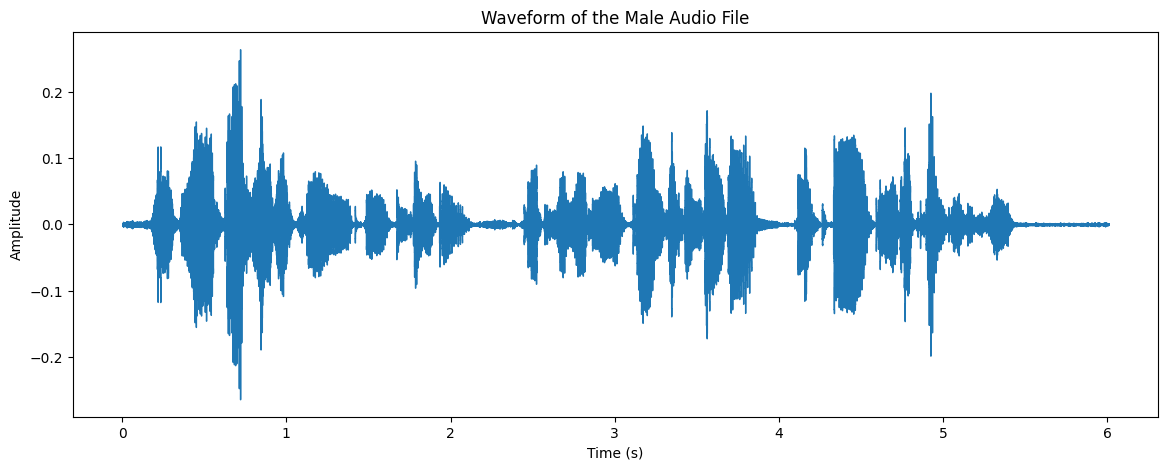
\includegraphics[width=3 in]{Dataset-Male.png}
    \caption{Male Audio Signal as Waveform}
    \label{fig:Dataset-Male}
\end{figure}

\begin{figure}
    \centering
    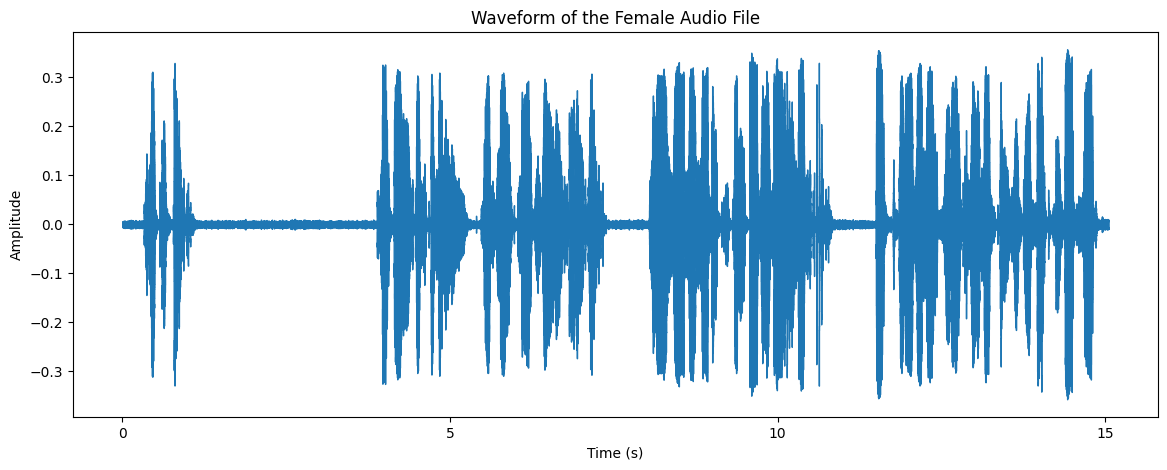
\includegraphics[width=3 in]{Dataset-Female.png}
    \caption{Female Audio Signal as Waveform}
    \label{fig:Dataset-Female}
\end{figure}

To improve the performance of these models, it is crucial to extract meaningful features from the voice recordings. This study utilizes several feature extraction techniques, including Mel-frequency cepstral coefficients (MFCC), delta MFCC, delta-delta MFCC (also known as 2 delta MFCC)~\cite{singh2014approach}, shifted delta coefficients~\cite{torres2002approaches}, pitch~\cite{yang2016pitch}, magnitude~\cite{kobayashi2014acoustic}, Filter-Bank Energies~\cite{tak2017novel}, and contrast features~\cite{arandjelovic2018objects}. MFCCs~\cite{singh2014approach} are widely used in speech recognition for their ability to capture the power spectrum of audio signals, while delta and delta-delta MFCCs help capture temporal dynamics. Shifted delta coefficients provide robustness to noise, and pitch features capture the fundamental frequency of the speech signal. Magnitude~\cite{kobayashi2014acoustic} features represent the energy distribution over different pitch classes, and contrast features highlight the difference in spectral peaks and valleys, which are useful for distinguishing between different types of sounds. Filter-Bank Energies~\cite{tak2017novel}, derived from applying filter banks to the power spectrum, offer a robust representation of the signal's energy distribution across different frequency bands, aiding in capturing diverse vocal characteristics.

This study seeks to provide a comprehensive evaluation of these architectures by comparing their performance on a standardized voice dataset. Through the analysis of metrics such as accuracy, precision, recall, and computational efficiency, this research aims to identify the most effective model for real-world applications. Additionally, the study explores the implications of model complexity, training time, and resource requirements, offering insights into the practical deployment of these technologies.

The document is organized into several key sections. Section II provides an extensive review of established models and research on the subject, offering valuable insights that help identify areas for improvement, gaps in current knowledge, and alternative strategies. This section also presents evidence supporting the effectiveness of the proposed solution or highlights possible challenges. Section III describes the implemented model, while Section IV outlines the dataset used for both testing and training. Section V summarizes the report's findings and includes a summary of results along with suggestions for future research directions.

The findings of this research are expected to contribute to the advancement of voice-based recognition systems by providing a detailed understanding of the strengths and limitations of each architecture. This comparative study will serve as a valuable resource for researchers and practitioners aiming to develop more accurate and efficient voice recognition systems tailored to specific demographic characteristics.
\section{Related work}

\section{Proposed Method}
\begin{figure}
    \centering
    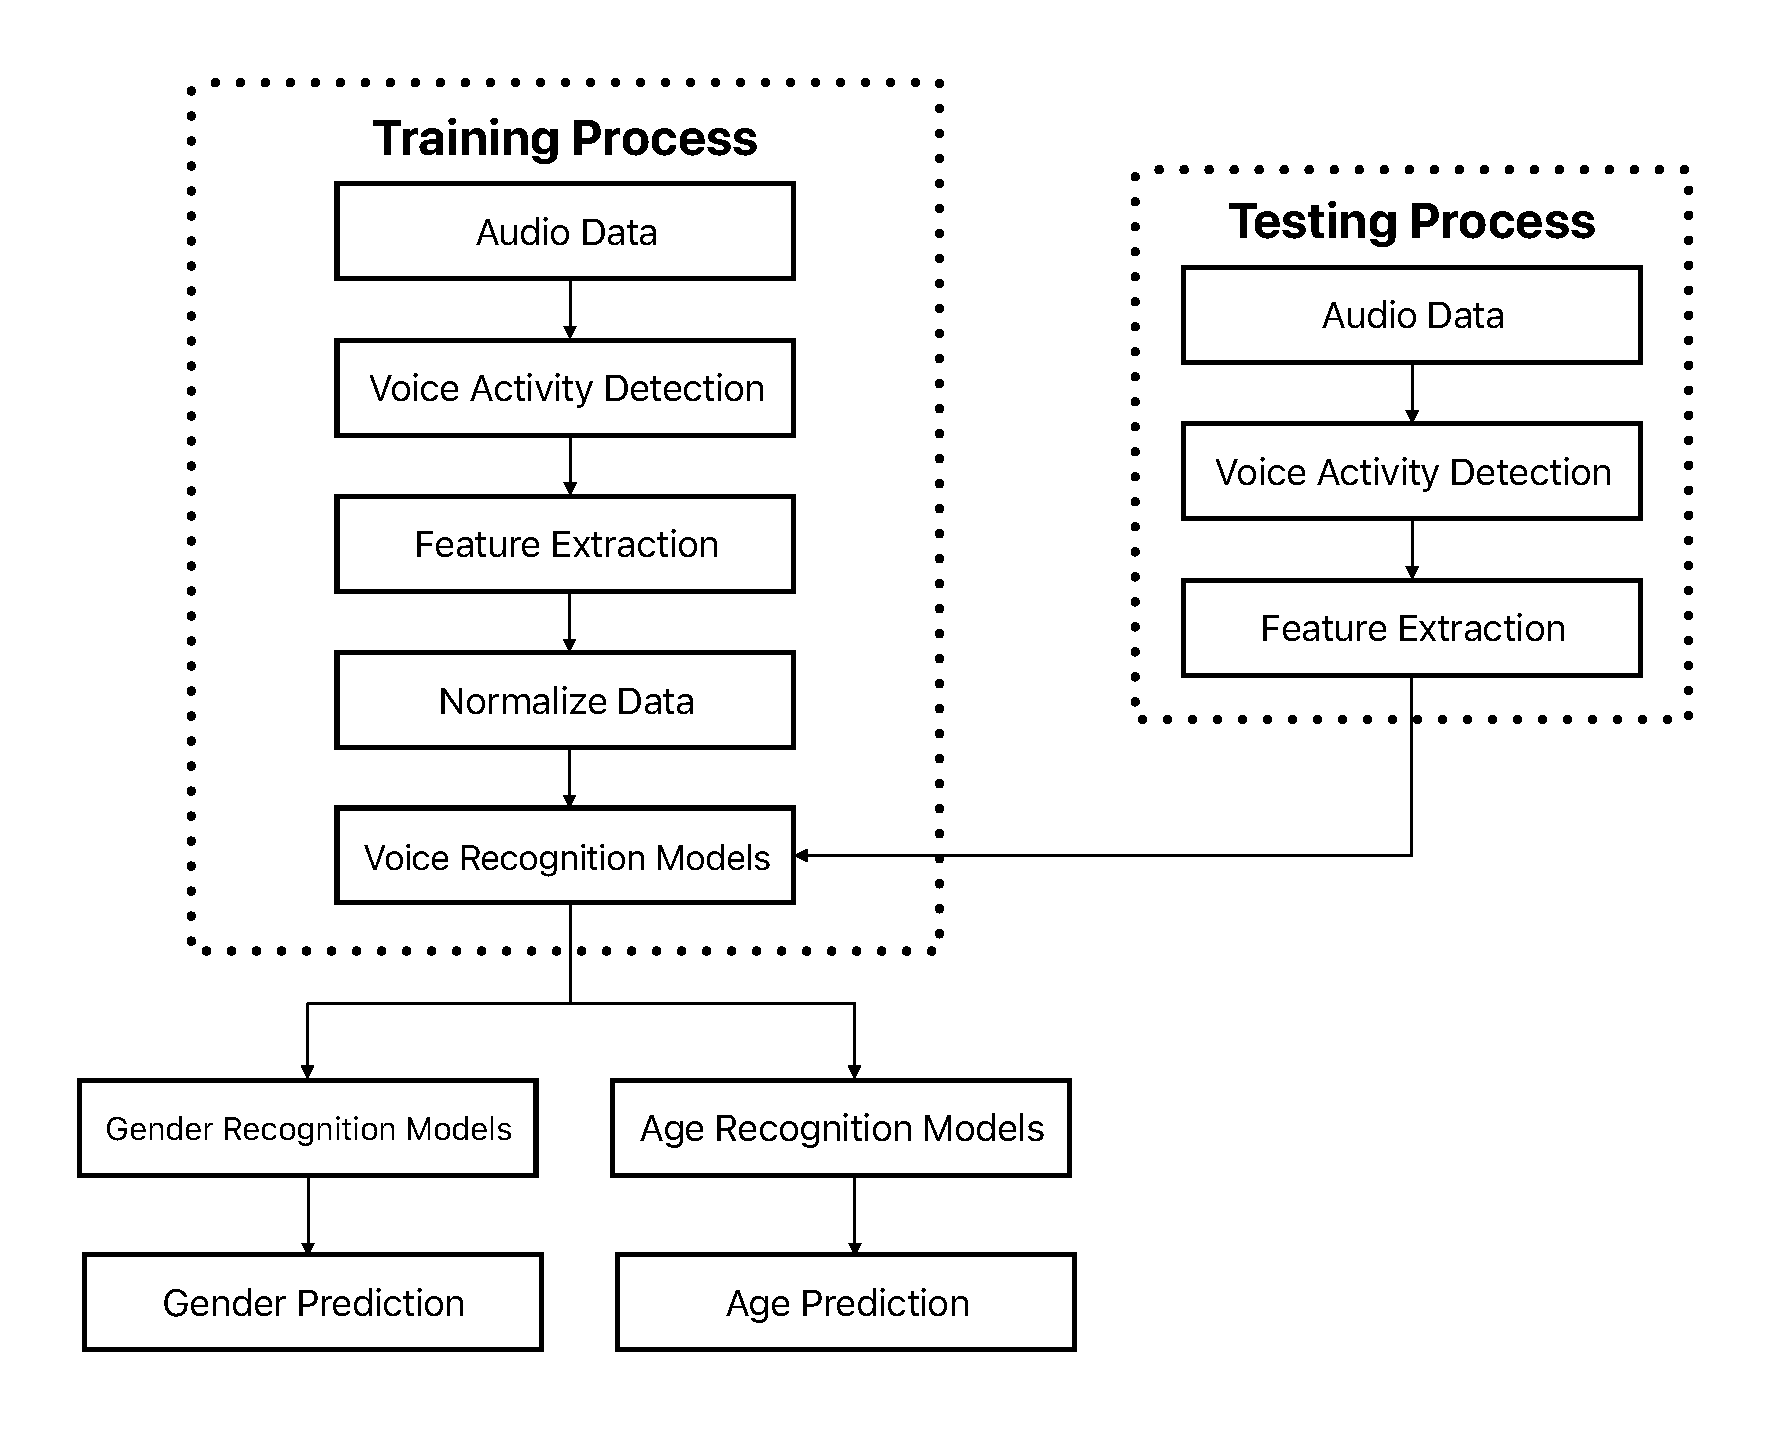
\includegraphics[width=3.5 in]{Research Architecture.pdf}
    \caption{Architecture of Recognition Model}
    \label{fig:Research Architecture}
\end{figure}
\subsection{Architecture}
\subsection{Sound Extraction}
\subsection{Performance Matrix}

\section{Experimental Result and Discussion}
\subsection{Experiment settings}

The training process is conducted on a personal computer equipped with an Intel® Core™ i7-12650H processor, and an NVIDIA GeForce RTX 3060 GPU with 8GB of RAM.
\subsection{Dataset}
\subsubsection{Dataset for Gender Recognition Model}

After The Mozilla Voice Dataset~\cite{mozilla_voice} cleansing procedures, we homogenized the dataset to solely include male and female classifications. Subsequently, we partitioned this refined dataset into subsets suitable for Gender Recognition Modeling, totaling %8,000
items. This allocation comprised %5,400
entries designated for training purposes, %600
for validation, and %2,000 
for testing. Notably, each subset maintained a balanced representation of genders, with male and female categories accounting for 50\% and 50\% of the data, respectively. It is represented through in Table~\ref{tab:Distribution of samples in the Gender dataset}.

\begin{table}[htbp]
    \centering
    \caption{Distribution of samples in the Gender dataset}
    \label{tab:Distribution of samples in the Gender dataset}
    \begin{tabular}{|c|ccc|}
    \hline
    \textbf{Category} & \textbf{Train Dataset} & \textbf{Valid Dataset} & \textbf{Test Dataset}\\
    \hline
    Male &  &  &  \\
    Female &  &  &  \\
    \hline
    \textbf{Total} &  &  & \\
    \hline
    \end{tabular}
\end{table}

\subsubsection{Dataset for Age Recognition Model}
 Following the Mozilla Voice Dataset~\cite{mozilla_voice} refinement processes, we standardized the dataset to encompass five age categories. Subsequently, we partitioned this refined dataset into subsets tailored for age-based modeling, totaling %8,000 
 items. This allocation included %13,279 
 entries designated for training purposes, %1,476 
 entries for validation, and %790 
 entries for testing. It is noteworthy that each subset retained a balanced representation across five age classifications: teens, twenties, thirties, forties, and fifties to sixties. It is represented through Table~\ref{tab:Distribution of samples in the Age dataset}.

\begin{table}[htbp]
    \centering
    \caption{Distribution of samples in the Age dataset}
    \label{tab:Distribution of samples in the Age dataset}
    \begin{tabular}{|c|ccc|}
    \hline
    \textbf{Category} & \textbf{Train Dataset} & \textbf{Valid Dataset} & \textbf{Test Dataset}\\
    \hline
    Teens &  &  & 160 \\
    Twenties &  &  & 160 \\
    Thirties &  &  & 160 \\
    Forties &  &  & 160 \\
    Fifties - Sixties &  &  & 160 \\
    \hline
    \textbf{Total} &  &  & 800\\
    \hline
    \end{tabular}
\end{table}
\subsection{Feature Extraction}
\subsection{Model}
\subsubsection{Support Vector Machine (SVM) architecture}
\subsubsection{Convolutional Neural Network (CNNs) architecture}
\subsubsection{Long - Short Term Memory (LSTMs) architecture}
\subsubsection{Bidirectional Long - Short Term Memory (BiLSTMs) architecture}
\subsubsection{RezoNet architecture}
\subsection{Comparison Architecture}

\section{Conclusion}

\bibliographystyle{IEEEtran}  % IEEE
\bibliography{Mybib}          % IEEE

\end{document}


